\documentclass[10pt]{article}
%%%%%%%%%%%%%%%%%%%%%%%%%%%%%%%%%%%%%%%%
\usepackage{amsmath}
\usepackage{verbatim}
\usepackage[usenames,dvipsnames]{color}
\usepackage{ulem}
\usepackage{setspace}
\usepackage{lscape}
\usepackage{longtable}
\usepackage[top=1.25in,bottom=1.5in,left=1in,right=1.5in,landscape]{geometry}
\usepackage{graphicx}
\usepackage{epstopdf}
\usepackage[usenames,dvipsnames]{pstricks}
\usepackage{epsfig}
\usepackage{pstricks-add}
\usepackage{pst-node}
\usepackage{fancyhdr}
\usepackage[absolute,showboxes]{textpos}

%TCIDATA{OutputFilter=LATEX.DLL}
%TCIDATA{Version=5.00.0.2552}
%TCIDATA{<META NAME="SaveForMode" CONTENT="1">}
%TCIDATA{Created=Thursday, August 28, 2003 13:38:44}
%TCIDATA{LastRevised=Thursday, August 14, 2008 15:20:27}
%TCIDATA{<META NAME="GraphicsSave" CONTENT="32">}
%TCIDATA{<META NAME="DocumentShell" CONTENT="Standard LaTeX\Blank - Standard LaTeX Article">}
%TCIDATA{Language=American English}
%TCIDATA{CSTFile=LaTeX article (bright).cst}

\setcounter{MaxMatrixCols}{10}

\newenvironment{proof}[1][Proof]{\noindent\textbf{#1.} }{\ \rule{0.5em}{0.5em}}
\setlength{\columnsep}{.2in}

\renewcommand{\labelitemii}{$\cdot$}

\pagestyle{fancy} \fancyhead{} \fancyfoot{} \rfoot{} \lfoot{}

\newcommand{\slide}[2]{
\begin{textblock}{11}(0,0)
\textcolor{Black}{\textbf{\huge \rule{0pt}{1in} \raisebox{.2in}{#1}}}
\end{textblock}
\begin{Large} \noindent
#2
\end{Large}
\vfill \pagebreak}

\setlength{\TPHorizModule}{1in}
\setlength{\TPVertModule}{1in}
\textblockcolour{Yellow}
\renewcommand{\headrulewidth}{0pt}



\begin{document}
\onehalfspacing 

\lfoot{Institutions} \rfoot{Economic Growth}

\slide{Big Questions}{What dictates:
\begin{itemize}
	\item The investment rate in new capital? ($s_K$)
	\item The investment rate in new human capital? ($u$)
	\item The adoption/discovery of new technologies? ($\mu$)
	\item The level of investment in innovation? ($s_R$)
\end{itemize}

\vspace{.25in}\noindent These factors all create level effects on output per worker. Why are some countries on a high level, while others remain on a low level?
}

\slide{Big Answers}{Several:
\begin{itemize}
	\item Geography. Easy access to certain resources makes it cheaper to invest/use them.
	\item Culture. Certain cultures value savings or education more than others.
	\item Institutions. Rules of the economic game, so to speak.
\end{itemize}

\vspace{.25in}\noindent Olson (1996) - compare several places identical in geography and culture
\begin{itemize}
	\item North vs. South Korea
	\item East vs. West Germany
	\item China vs. Taiwain and Hong Kong
\end{itemize}
They differ in institutions. 
}

\slide{Investment Problem}{How do we think of institutions?
\begin{itemize}
	\item Property rights: the ability to keep what you earn in profits, savings, wages
	\item Transactions: the ability to easily trade assets, sign contracts
	\item Enforcement: contracts and laws are enforced consistently over time
\end{itemize}

\vspace{.25in}\noindent The overall point is that ``good'' institutions will encourage people to invest because they can keep what they earn and they can make long-run investments because the rules won't arbitrarily change over time.
}

\slide{Practical Evaluation}{How do we think of this with respect to our existing model. Think of the value of a patent (or value of contract to produce certain intermediate good)
\begin{equation}
P_A = \frac{\pi}{r-n}
\end{equation}
is the present discounted value of the profits. The value of this dictates how much effort goes into innovating or adopting technology - $s_R$.

\vspace{.25in}\noindent Think of institutions as how they play with this value. Let there be some fixed cost that you have to pay if you buy the patent, $F$, so now $P_A$ is
\begin{equation}
P_A = \frac{\pi}{r-n} - F
\end{equation}
In the book, we call $\Pi = \pi/(r-n)$, but same idea.
}

\slide{Fixed Costs}{What could make up fixed costs, $F$?
\begin{itemize}
	\item License fees
	\item Bribes
	\item Protection money
	\item Rights to market in some area
	\item Taxes
\end{itemize}

\vspace{.25in}\noindent Anything that raises $F$, the fixed cost of owning the patent, will drive down the value of a patent, $P_A$. The lower $P_A$, the less innovation/adoption we do, $s_R$ drops.
}

\slide{Doing Business}{World Bank collects data on how long it takes to set up businesses, and cost in terms of licenses, fees, etc..
\begin{itemize}
	\item U.S.: six days and equivalent 1.4\% of average income
	\item India: 29 days and equivalent 50\% of average income
	\item Nigeria: 34 days and equivalent 70\% of average income
	\item Honduras: 14 days and equivalent 63\% of average income
\end{itemize}

\vspace{.25in}\noindent It is not trivial to start new firms, invest in new equipment, adopt a new technology in most poor countries. 
}

\slide{Corruption}{
\begin{quote}
	To invest in a Russian company, a foreigner must bribe every agency involved in foreign investment, including the foreign investment office, the relevant industrial ministry, the finance ministry, the executive branch of the local government, the legislative branch, the central bank, the state property bureau, and so on. The obvious result is that foreigners do not invest in Russia. Such competing bureaucracies, each of which can stop a project from proceeding, hamper investment and growth around the world, but especially in countries with weak governments. 
\end{quote}
Shleifer and Vishny 1993, pp. 615–16.

}

\slide{Profits}{Institutions also affect the scale of profits.
\begin{itemize}
	\item Larger markets (more $L$) means more profits
	\item Barriers to trade limit market sizes, reduce profits
	\item Lower profits means less innovation
\end{itemize}

\vspace{.25in}\noindent Rich places:
\begin{itemize}
	\item U.S.: Can sell in any state with minimal or no additional requirements
	\item E.U.: Joins many small countries together into one big market
\end{itemize}

}

\slide{Social Infrastructure}{How do you measure institutions?
\begin{itemize}
	\item You don't, not directly
	\item Surveys of business conditions
	\item Evaluations by agencies of costs of doing business
	\item Very rough rankings of countries
\end{itemize}

\vspace{.25in}\noindent We use a measure of ``social infrastructure'' that captures six dimensions of governance from the World Bank
\begin{itemize}
	\item Accountability of politicians
	\item Political stability
	\item Government effectiveness
	\item Regulatory quality
	\item Rule of law
	\item Control of corruption
\end{itemize}
Overall index runs from 0 (worst) to 1 (best)
}

\slide{Savings and Institutions}{
\begin{center}
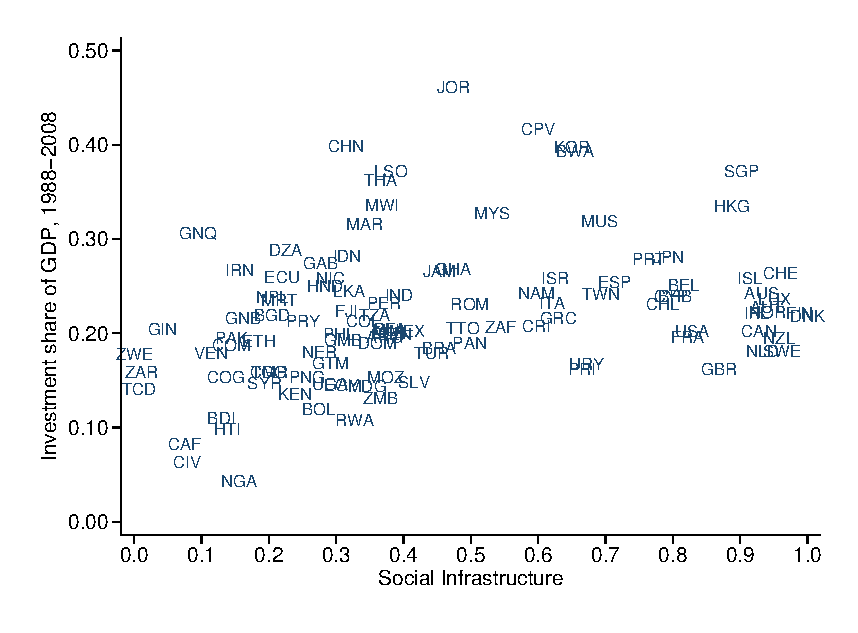
\includegraphics[scale=1.3]{figure_7_1.eps}
\end{center}
}

\slide{Human Capital and Institutions}{
\begin{center}
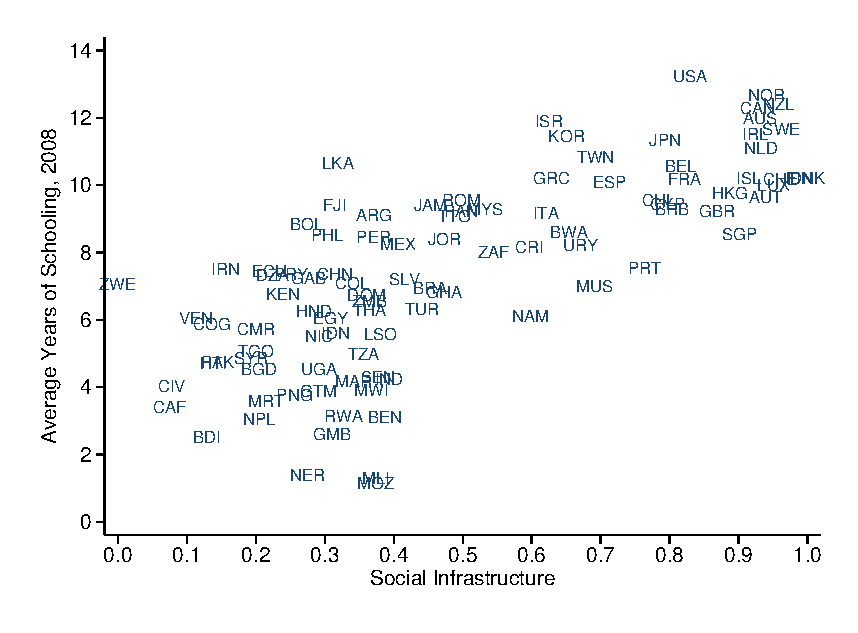
\includegraphics[scale=1.3]{figure_7_2.eps}
\end{center}
}

\slide{TFP and Institutions}{
\begin{center}
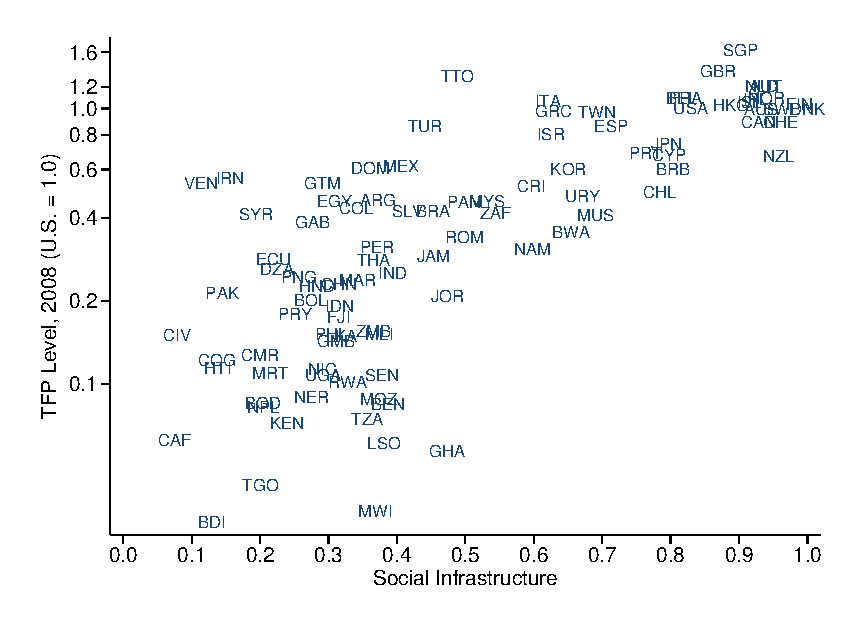
\includegraphics[scale=1.3]{figure_7_3.eps}
\end{center}
}

\slide{Choosing Institutions}{If good institutions generate big economic gains, why don't all countries have them?
\begin{itemize}
	\item Institutions are human-designed and malleable
	\item Can't we bargain with each other to get good institutions?
	\item Can't elites take smaller slice of a bigger pie?
	\item Example: offer beauracrats higher salaries in exchange for not taking bribes
\end{itemize}

\vspace{.25in}\noindent Acemoglu and Robinson (2005,2012) say we cannot because of commitment problems.
\begin{itemize}
	\item The beauracrats will take higher salary, and then still ask for a bribe
	\item Elites cannot credibly promise to take smaller slice.
	\item Non-elites cannot credibly promise not to replace elites.
\end{itemize}

\vspace{.25in}\noindent Institutions appear to be very persistent, and historically contingent

}

\end{document}